\chapter{Stworzenie gry}
\thispagestyle{chapterBeginStyle}
\label{rozdzial1}

\SetKwComment{Comment}{/* }{ */}

\subsection{Cel i funkcjonalności}
Gra została stworzona przede wszystkim jako środowisko treningowe oraz testowe bota, dopiero w drugiej kolejności jako rozrywka dla użytkownika. Dostarczona w dodatku $A$ gra pozwala graczowi na załadowanie jednego z domyślnych terenów, bądź stworzenie własnego terenu i przetestowanie go w grze. Celem rozgrywki jest przetransportowanie pojazdu od miejsca startowego do mety, nie zjeżdżając ze ścieżki. Gra kończy się po wykonaniu jednego pełnego okrążenia. Gracz konkuruje z 3 innymi pojazdami, sterowanymi przez wytrenowanego bota. Dodatkowo gracz posiada możliwość stworzenia własnego terenu i trasy, sterując kilkoma parametrami. W ten sam sposób zostały przygotowane tereny, na których został wytrenowany bot.

\subsection{Wykorzystane technologie}
Gra została stworzona z wykorzystaniem silnika do gier Unity Engine 3D. Jest to jeden z dwóch najpopularniejszych silników do tworzenia gier, poza Unreal Engine, natomiast posiada on niższą barierę wejścia. Wykorzystanie Unity pozwoliło na zasymulowanie praw fizyki występujących przy prowadzeniu pojazdu.

\subsection{Stworzenie trasy 2D}
Pierwszym etapem generowania terenu jest wybór krzywej opisującej trasę. Każda wygenerowana trasa jest krzywą zamkniętą. Składa się ona z segmentów, których ilość jest bezpośrednio powiązana z zawiłością trasy. 

Aby wybrać końce segmentów, losowane są punkty $P=(P_x,P_y)$ na płaszczyźnie z uniwersalnym prawdopodobieństwem, z zakresu $P_x \in [-1, 1]$, $P_y \in [-1, 1]$, upewniając się że żadne 2 punkty nie są za blisko siebie.
\\\phantom{.}\\
\begin{algorithm}[H]
\caption{Wybór punktów trasy}\label{alg:two}
\KwData{\\
    $n \gets$ \textit{ilość segmentów}\;
    $d \gets$ \textit{minimalna odległość między punktami}\;}
$positions \gets []$\;
\While{$positions.Length < n$}{
    $pNew \gets$ \textit{new point}\;
    $pNew.x \gets random(-1, 1)$\;
    $pNew.y \gets random(-1, 1)$\;
    $tooClose \gets false$\;
    \ForEach{$P \in positions$}{
        \If{$distance(P, pNew) < d$}{
            $tooClose \gets true$\;
            $break$\;
        }
    }
    \If{\textit{not tooClose}}{
        \textit{add pNew. to positions}\;
    }
}
\end{algorithm}
\phantom{.}\\
Po wyborze odpowiedniej ilości punktów, sortowane są one zgodnie z ruchem wskazówek zegara, na podstawie kąta pomiędzy wektorem $[0, 1]$, a wektorem kończącym się w danym punkcie.
\\\\
\begin{algorithm}[H]
    \caption{Wyznaczenie kąta pomiędzy punktem a prostą OY}\label{alg:two}
    \KwData{$P \gets$ \textit{punkt}}
    $forwardVector \gets [0, 1].normalized$\;
    $pointVector \gets [P.x, P.y].normalized$\;
    $angle \gets acos(dot(forwardVector, pointVector))$ \Comment*[r]{Arcus cosinus iloczynu skalarnego}
    $sign \gets cross(forwardVector, pointVector).z$ \Comment*[r]{iloczyn wektorowy}
    \eIf{$sign \geq 0$}{
        \Return{$angle$}\;
        } {
        \Return{$-1 \cdot angle$}\;
    }
\end{algorithm}
\phantom{.}\\
Następnie trasa w każdym segmencie wyznaczana jest za pomocą krzywej Bezier 3 stopnia, ponieważ pozwala ona w stosunkowo prosty sposób zapisać stosunkowo komplikowane krzywe, utrzymując płynny kształt. Każda krzywa Bezier składa się z punktu startowego $P_0$, końcowego $P_3$, oraz dwóch punktów kontrolnych $P_1$, $P_2$, oraz wyraża sie wzorem:
\[ b(t) = (1 - t)^3 * P_0 + 3t(1-t)^2 * P_1 + 3t^2 (1-t) * P_2 + t^3 * P_3 \hspace{1cm}\textit{dla } t \in [0, 1] \]
Aby zapewnić płynne połączenia pomiędzy segmentami, sąsiednie punkty kontrolne powinny znajdować sie na tej samej prostej. Dla każdego punktu startowego wyznaczane są punkty kontrolne segmentu poprzednioego i następnego, na podstawie sąsiadujących punktów startowych.

Poniższy rysunek przedstawia trzy wylosowane punkty $A,B,C$, oraz proces generacji punktów kontrolnych dla środkowego punktu $B$. Na początku wyznaczana jest prosta prostopadła do dwusiecznej kąta pomiędzy wektorami $BA$ i $BC$, poprzez normalizację ww. wektorów odpowiednio do $BA'$ i $BC'$, a następnie odjęcie powstałych wektorów. Punkt kontrolny $D$ znajduje się na ww. prostej, w odległości równej połowie długości wektora $BA$. Analogicznie położony jest punkt kontrolny $E$. Po wykonaniu powyższych operacji dla każdego punktu startowego na wyznaczonej trasie, w każdym segmencie znajdują się oba punkty kontrolne. Po podstawieniu punktów startowych i kontrolnych (np. $A,F,D,B$) dla każdego segmentu wyznaczona zostanie cała trasa.

\begin{figure}[h]
    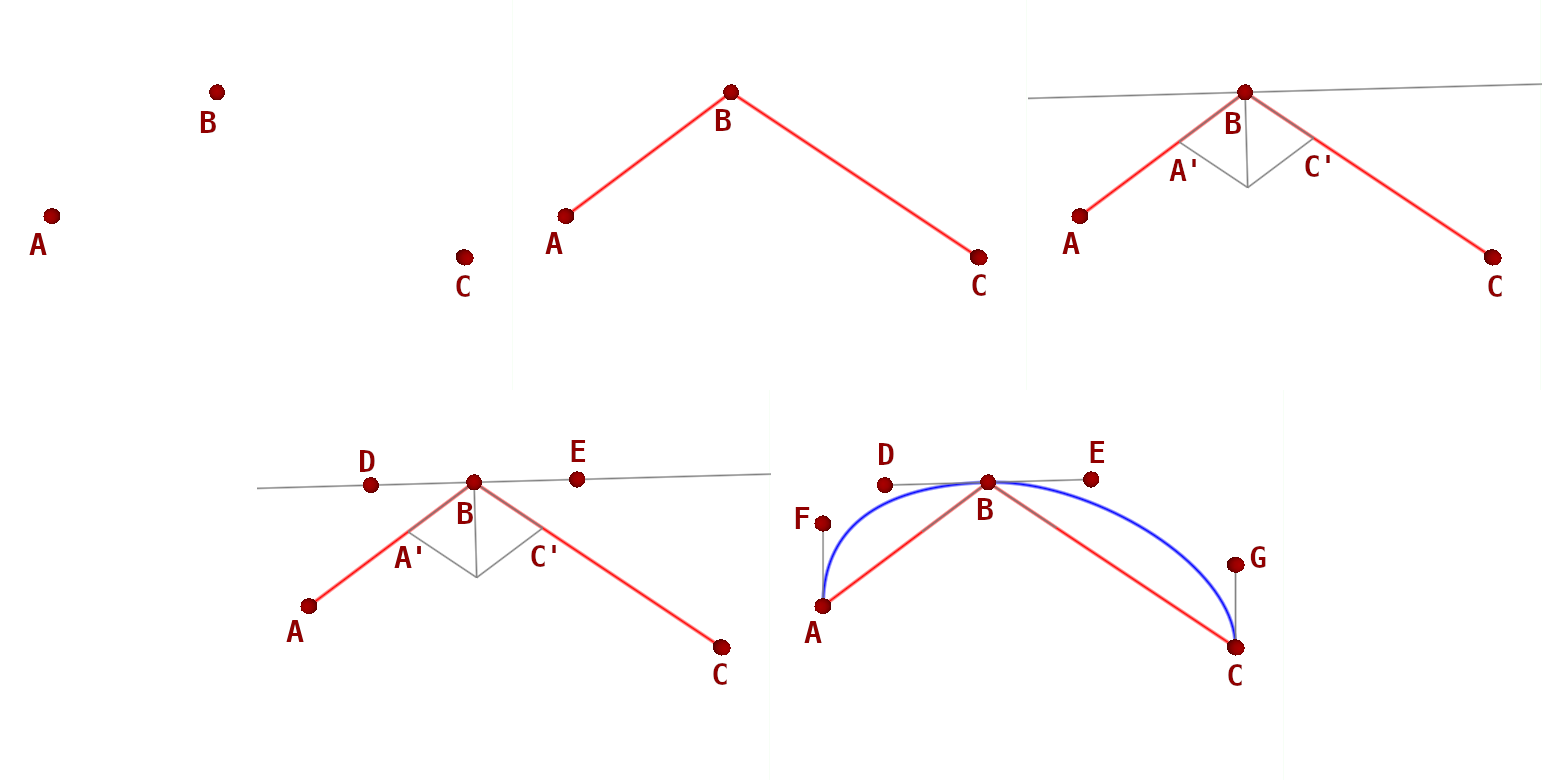
\includegraphics[width=\textwidth]{figures/loop_creation}
    \caption{Generowanie punktów kontrolnych krzywej Bezier}
    \label{fig}
\end{figure}

\subsection{Stworzenie terenu 3D}
Każdy stworzony teren gry jest rozmiaru $512 x 512$, z czego $10\%$ przeznaczone jest na marginesy z każdej strony, co pozostawia wewnętrzną przestrzeń $409 x 409$ na wygenerowany tor. Każdy punkt wygenerowanej pętli jest skalowany odpowiednio, aby trasa wypełniła całość dostępnej przestrzeni. Następnie dla każdego punktu terenu generowana jest wysokość, zdefiniowana jako procent maksymalnej wysokości $128$. Wysokość składa się z trzech warstw, wykorzystujących Szum Perlina, każda coraz bardziej szczegółowa. Implementacja Szumu Perlina została dostarczona jako fragment biblioteki $Mathf$ przez Unity \cite{PerlinNoise}.
\\\\
\begin{algorithm}[H]
    \caption{Wyznaczenie wysokości terenu}\label{alg}
    \KwData{\\
        $x \gets$ \textit{wspołrzędna X punktu}\;
        $y \gets$ \textit{wspołrzędna Y punktu}\;}
    $x \gets x + offsetX$\;
    $y \gets y + offsetY$\;
    $h1 \gets detailsMain \cdot PerlinNoise(x \cdot scaleMain, y \cdot scaleMain)$\;
    $h2 \gets detailsMinor \cdot PerlinNoise(x \cdot scaleMinor, y \cdot scaleMinor)$\;
    $h3 \gets detailsTiny \cdot PerlinNoise(x \cdot scaleTiny, y \cdot scaleTiny)$\;
    \Return{h1 + h2 + h3}
\end{algorithm}
\phantom{.}\\
Powyższa funkcja pozwala na sterowanie krztałtem terenu poprzez parametry $details$ i $scale$ dla każdej z trzech warstw $main$, $minor$, $tiny$. Warstwa $main$ definiuje ogólny krztałt terenu, warstwa $minor$ dodaje mniejsze pagórki, natomiast warstwa $tiny$ dodaje drobne detale. Dodatkowo poprzez sterowanie $offsetX$ i $offsetY$ możliwe jest przesunięcie wszystkich wartości w płaszczyźnie poziomej.

\subsection{Przypisanie tekstur}
Zależnie od rodzaju terenu, wybierany jest odpowiedni zestaw tekstur. Dla każdego punktu wygenerowanego terenu przypisane są odpowiednie wartości przezroczystości tekstur, tworząc jak najbardziej realistyczne krajobrazy. Decyzja o wybraniu przezroczystości tekstur została podjęta na podstawie rodzaju terenu wybranego przez użytkownika, wysokości danego punktu, kierunku płaszczyzny zbocza, kąta nachylenia zbocza oraz odległości punktu od centrum wygenerowanej trasy. Odczytanie wartości takich jak wysokość, kierunek płaszczyzny i kąt nachylenia można wykonać w stałym czasie $O(1)$. Natomiast znalezienie najbliższego punktu trasu jest bardziej złożonym procesem. Poniżej przedstawiono proces wyboru metody jego wyznaczania.

\subsection{Znalezienie najbliższego punktu krzywej Bezier}
Poniższa metoda dzieli każdy segment trasy na $m$ odcinków, a następnie iteruje wszystkie końce odcinków we wszystkich segmentach. Optymalna ilość podziału wyznaczona została eksperymentalnie. Metoda ta ma złożoność czasową $O(nm)$, gdzie $n$ oznacza liczbę segmentów trasy, natomiast $m$ oznacza dokładność podziałów danego segmentu.
\\\\
\begin{algorithm}[H]
    \caption{Znalezienie najbliższego punktu krzywej Bezier}\label{alg}
    \KwData{$P \gets$ \textit{cel poza krzywą}}
    $minDist \gets infinity$\;
    $minT \gets 0$\;
    \For{i = 0; i < 100; i++}{
        $t \gets i \cdot 0.01$\;
        $pProjection \gets B(t)$ \Comment*[r]{punkt w t\% długości krzywej bezier}
        $dist \gets distance(P, pProjection)$\;
        \If{dist < minDist}{
            $minDist \gets dist$\;
            $minT \gets t$\;
        }
    }
    \Return{B(minT)}
\end{algorithm}
\phantom{.}\\

\subsection{Udoskonalone znalezienie najbliższego punktu krzywej Bezier}
Poniższa metoda wywodzi się z artykułu \cite{ImprovedPointProjectionBezier}, oraz została przystosowana dla krzywej Bezier 3 stopnia.\\
Funkcja opisująca krzywą Bezier:
\[ b(t) = (1 - t)^3 P_0 + 3t(1-t)^2 P_1 + 3t^2 (1-t) P_2 + t^3 P_3 \]
Pierwsza pochodna po t:
\[ \frac{b}{dt}(t) = -3 (1 - t)^2 P_0 + 3 (1-t)^2 P_1 - 6 t (1-t) P_1 - 3t^2 P_2 + 6 t (1-t) P_2 + 3t^2 P_3 \]
Aby znaleźć rzut celu na krzywą, zależy znaleźć taki punkt na krzywej, aby styczna w tym punkcie była prostopadła do odcinka łączącego go z celem. Zatem dla zadanego punktu celu $C$ i szukanej wartości $t$, określającej w którym miejscu krzywej znajduje się szukany rzut, zdefiniowana została funkcja $f$:
\[ f(t) = (C - b(t)) \cdot \frac{b}{dt}(t) \]
Funkcja $f$ wykorzystuje iloczyn skalarny, zatem szukane $t$ zwraca wartość $f(t) = 0$. Ze względu na kształt krzywej, może na niej znajdować się kilka punktów będących rzutami prostopadłymi celu $C$, natomiast poszukiwany jest punkt najbliżej celu, zatem funkcję $f$ należy przemnożyć przez odległość od celu do znalezionego punktu.
\[ f(t) = \big[ (C - b(t)) \cdot \frac{b}{dt}(t) \big] distance(C, b(t)) \]
Aby znaleźć najbliższy punkt na krzywej, należy znaleźć miejsce zerowe funkcji $f(t)$. W tym celu wykorzystano zmodyfikowaną metodę bisekcji. Tradycyjnie metoda bisekcji zakłada, że wartości funkcji na obu krańcach przedziału są przeciwnego znaku, następnie wybiera środkowy punkt i kontynuuje przeszukiwanie już w połowie przedziału. Natomiast w tym wypadku nie jest zagwarantowane, że funkcja będzie miała przeciwne znaki na końcach przedziału, dlatego gdy są tego samego znaku, liczona jest bisekcja dla obu podprzedziałów.
\\\\
\begin{algorithm}[H]
    \caption{Udoskonalona bisekcja}\label{alg}
    \KwData{\\
        $a \gets$ \textit{początek przedziału}\;
        $b \gets$ \textit{koniec przedziału}\;
        $delta \gets$ \textit{dokładność argumentów}\;
        $epsilon \gets$ \textit{dokładność wyników}\;
        $maxit \gets$ \textit{maksymalna ilość iteracji}\;}
    \If{$maxit < 1$}{
        \Return{(a+b)/2}
    }
    $u \gets f(a)$\;
    $v \gets f(b)$\;
    $e \gets (b-a)/2$\;
    $c \gets a+e$\;
    $w \gets f(c)$\;
    \eIf{sing(u) != sign(v)}{
        \If{$abs(e) < delta$ or $abs(w) < epsilon$}{
            \Return{c}
        }
        \eIf{sing(u) != sign(w)}{
            \Return{UdoskonalonaBisekcja(a, c, delta, epsilon, maxit - 1)}
        }{
            \Return{UdoskonalonaBisekcja(c, b, delta, epsilon, maxit - 1)}
        }
    }{
        $left \gets UdoskonalonaBisekcja(a, c, delta, epsilon, maxit / 2)$\;
        $right \gets UdoskonalonaBisekcja(c, b, delta, epsilon, maxit / 2)$\;
        \eIf{$abs(f(left)) < abs(f(right))$}{
            \Return{left}
        }{
            \Return{right}
        }
    }
\end{algorithm}
\phantom{.}\\

\subsection{Porównanie metod}
Metoda druga jest wykonywana szybciej, dodatkowo zapewniając większą szczegółowość.
\begin{table}[h]
    \centering
    \begin{tabular}{|c|c|c|c|c|c|}
        \hline
        \multicolumn{2}{|c|}{Method 1} & \multicolumn{3}{c|}{Method 2} & lp\\
        ilość podziałów & czas [ms] & ilość iteracji & odpowiadająca ilość podziałów & czas [ms] & \\
        \hline
        \hline
        50 & 42046 & 5 & $2^{5}=32$ & 30580 & 1 \\
        100 & 81421 & 10 & $2^{10}=1024$ & 59606 & 2 \\
        150 & 121224 & 15 & $2^{15}=32768$ & 70178 & 3 \\
        \hline
    \end{tabular}
    \caption{Porównanie metod rzutowania punktu na krzywą Bezier}
    \label{table}
\end{table}
\clearpage

\subsection{Optymalizacja czasu}
Zastosowanie wybranej metody dla każdego z $1048576$ punktów (przy rozdzielczości terenu $1024 x 1024$) trwa ponad godzinę i produkuje dużą liczbę nieużywanych informacji. Aby skrócić czas generowania terenu do minimum teren został podzielony na sekcje. Następnie, jeżeli środkowy punkt sekcji znajdował się w odległości od drogi mniejszej niż połowa przekątnej sekcji, tj. jeżeli droga przebiegała przez daną sekcję, była ona rekurencyjnie dzielona na podsekcje. Powyższe kroki powtórzono aż do otrzymania zadowalającej jakości.
\begin{figure}[h]
    \centering
    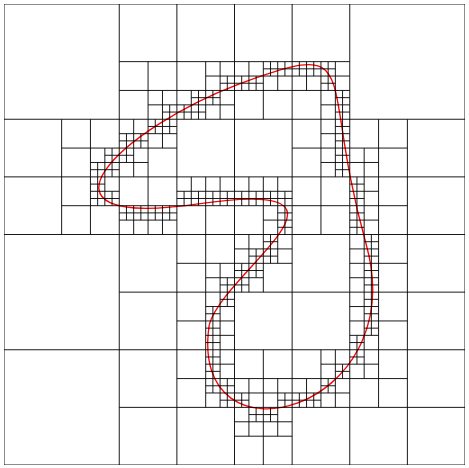
\includegraphics[width=0.5\textwidth]{figures/terrain_subdivision_for_road}
    \caption{Podział terenu w celu optymalizacji ilości obliczeń}
    \label{fig}
\end{figure}

\subsection{Dodanie obiektów}
Ostatnim etapem jest dodanie obiektów, takich jak meta oraz pojazdy. Domyślnie na każdym torze znajdą się cztery pojazdy, ustawione jeden za drugim, z czego trzy sterowane przez bota, a jeden przez gracza. Dodatkowo dodawane są krawędzie, których celem jest zapobieganie spadania pojazdu poza wygenerowany teren. W celu śledzenia przebiegu trasy, w równych odstępach dodawane są punkty kontrolne.\\
Przykładowo otrzymano poniższy efekt:
\begin{figure}[h]
    \minipage{.5\textwidth}
        \centering
        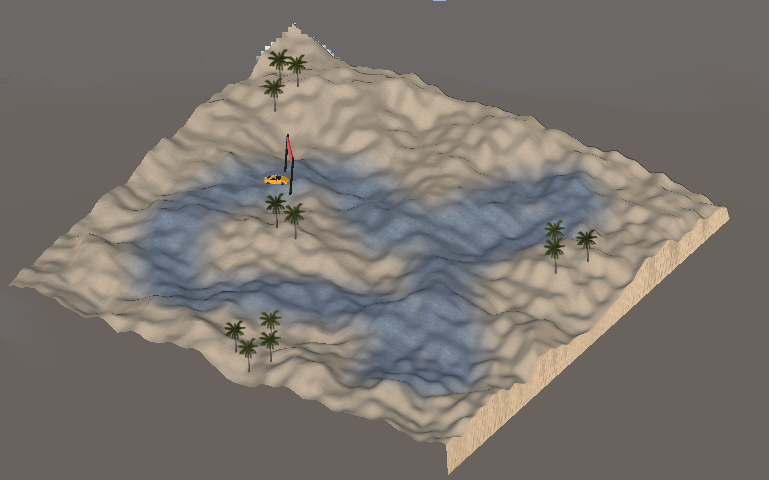
\includegraphics[height=5cm]{figures/terrains_2.png}
    \endminipage\hfill
    \minipage{.5\textwidth}
        \centering
        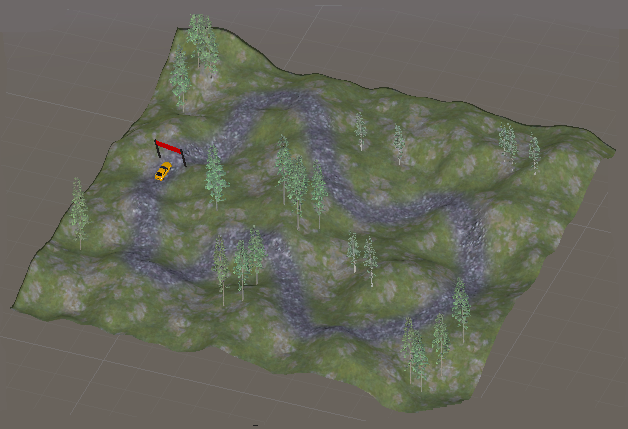
\includegraphics[height=5cm]{figures/terrains_1.png}
    \endminipage
    \caption{Wygenerowane tereny}
    \label{table}
\end{figure}
\clearpage